\documentclass[preprint,12pt]{elsarticle}

\usepackage[T1]{fontenc}
\usepackage[utf8]{inputenc}
\usepackage{graphicx}
\usepackage{booktabs}
\usepackage{amsmath}
\usepackage{url}
\usepackage{lineno}

\graphicspath{{figures/}}
\biboptions{numbers,sort&compress}
\modulolinenumbers[1]

\journal{International Journal of Critical Infrastructure Protection}

\begin{document}

\begin{frontmatter}

\title{Digital Twins for Cyber-Resilient Power Grids: A Systematic Review and a
Research Agenda for the AI-Powered Era}

%% PLACEHOLDER — finalise author list and the corresponding author before submission.
%% The Research4Life Group A waiver attaches to the Bangladesh affiliation; a
%% corresponding author based outside Bangladesh forfeits the no-cost route.
\author[1]{Author One\corref{cor1}}
\ead{author.one@example.edu.bd}
\author[1]{Author Two}
\cortext[cor1]{Corresponding author.}

\affiliation[1]{organization={Department of Electrical and Electronic Engineering,
    University Name},
  city={Dhaka},
  country={Bangladesh}}

\begin{abstract}
Digital twins are becoming the reference architecture for monitoring, protecting and
controlling modern power grids, and artificial intelligence (AI) is being adopted inside
those twins at speed. We review whether the security literature treats AI as a defensive
tool faster than it models AI-enabled threats, or the twin itself, as an attack target.
Following PRISMA 2020 style, we screened 1,287 unique OpenAlex records, widened by four
adversarial-AI probe queries to a candidate pool of roughly 2,000, and retained 100
studies on digital twins for power-grid cybersecurity (2020--2026); 83 were coded
at full text across 46 fields and 17 at abstract level. The review is restricted to
power-grid papers that name a digital twin and a security term.
AI is used defensively in 70 of 83 full-text studies, while 35/83 (42.2\%) engage any
AI-enabled threat and 11/83 (13.3\%) engage one substantively; 48 (57.8\%) do not engage
at all. The twin itself is treated as an attack target in at most one study under a
strict codebook definition (a vehicle-twin review); the count under a looser
asset-under-protection definition is uncomputed. Threat coverage, as coded, concentrates
at operation (66/83; lifecycle-stage coder agreement $\kappa = 0.32$), with one
design-phase study and none at commissioning. In a 20\% blind sample, two coders agreed
on any-versus-none engagement at $\kappa = 0.60$ (16/20) and on substantive-versus-not
at $\kappa = 0.14$ (one shared substantive label of six); the corpus-level figures are
therefore bounds, not population estimates. We close with a five-item research agenda
in which every item is tied to the gap it addresses and the evidence that would confirm
it.
\end{abstract}

\begin{keyword}
digital twin \sep power grid \sep cyber-physical security \sep adversarial machine learning
\sep systematic review \sep research agenda
\end{keyword}

\end{frontmatter}

\linenumbers

\section{Introduction}

Electric power grids are digitising faster than they are being secured. Wide-area measurement,
distributed energy resources, electric-vehicle charging and market-coupled control have turned
the grid into a cyber-physical system whose behaviour is increasingly mediated by software
\cite{ref1,ref3}. The digital twin---a synchronised, bidirectional virtual counterpart of a
physical asset, updated from live sensor streams---has moved in the same decade from concept to
a reference architecture for grid monitoring, protection and control \cite{ref16,ref50}. That
same synchronisation is what makes the twin valuable and what makes it a target.

Artificial intelligence (AI) has followed the twin into the grid. Machine learning now performs
state estimation, anomaly detection, load and attack forecasting, and increasingly control
\cite{ref24,ref54}. The security community has been quick to adopt it. The question this review
asks is whether the same community has been as quick to model AI---and the twin itself---as
something an adversary can attack. Throughout, `digital twin' must be named by the authors, so
adversarial-ML work on grid security that does not mention a twin is out of scope and is not
represented in any figure here.

Early reading suggested a specific, testable asymmetry: grid digital-twin security research
adopts AI as a defensive tool far faster than it models AI, or the twin, as an attack target.
This review quantifies that asymmetry across a screened corpus and turns it into a research
agenda. It is a theory-testing systematic review, not an empirical deployment study.

\subsection{Positioning against prior reviews}

The closest work, and the reason this review had to be repositioned, is Habeeb, Weli and
Almaliki's 2026 PRISMA review of ``Dual-Role Digital Twins'' in cyber-physical security
\cite{habeeb2026}. Their contribution is real and prior: they name the dual role---the twin as
both an expanded attack surface and a defence enabler---and set out four research directions
around it. Their corpus is 20 studies, gathered with a query that has no specific attack operator,
and spread across manufacturing, healthcare, IIoT, smart city and water management, with the
power grid represented in roughly one study.

We therefore do not claim to have discovered the dual-role tension. Our position is narrower and
complementary. Habeeb et al.\ name two axes; we test a narrower, grid-side instance of the
attack-surface axis---with a published corpus, a closed threat vocabulary, and reported coder
reliability, but only where a grid twin is explicitly an attack target. In other words, they build
the theory; we report a lower bound on its grid manifestation, not a test of the full axis. Section~\ref{sec:related} sets out the mapping in full, including the five attack vectors their
review identifies and our corpus's coverage of them.

\subsection{Contributions}

\begin{enumerate}
  \item A PRISMA-2020-style corpus of 100 studies on digital twins for power-grid cybersecurity,
  screened from 1{,}287 unique records with a query set that includes explicit adversarial-AI
  probes (Section~\ref{sec:method}).
  \item A 46-field extraction of that corpus, coded by computer-assisted human reading, with
  the extraction method disclosed rather than hidden (Section~\ref{sec:method}).
  \item A two-coder reliability study on a 20\% blind sample, reported field by field including
  the fields where agreement is only fair (Section~\ref{sec:reliability}).
  \item The headline measurement: AI is defensive in 70/83 studies; 35/83 engage any AI-enabled
  threat and 11/83 engage one substantively, while the twin is explicitly named an attack target
  in one study (Section~\ref{sec:ai-threats}).
  \item A lifecycle concentration result: under a single-assigned lifecycle label, 66/83 studies sit
  at the operation phase (Section~\ref{sec:lifecycle}).
  \item A mapping from our independent threat vocabulary to the five vectors of
  Habeeb et al.\ \cite{habeeb2026}, showing coverage (vocabulary-level) plus six additional
  terms that their query could not return (Section~\ref{sec:related}); this is coverage,
  not evidence that the vectors are dealt with empirically.
  \item A five-item research agenda in which every item is tied to the gap that justifies it and
  the evidence that would validate it (Section~\ref{sec:agenda}).
\end{enumerate}

\subsection{Research questions}

\begin{description}
  \item[RQ1] How is the digital twin positioned in grid cybersecurity research---as a defensive
  tool, an attack target, or both?
  \item[RQ2] Which threats are named, at which grid domains and lifecycle stages, and with what
  threat models?
  \item[RQ3] How far does the corpus engage AI-enabled threats (adversarial machine learning,
  evasion, poisoning, LLM-specific, agentic)?
  \item[RQ4] How rigorous is the evidence base---evaluation method, maturity, baselines,
  metrics, and released code or data?
  \item[RQ5] What are the resulting gaps, and what would close them?
\end{description}

\subsection{Structure}

Section~\ref{sec:background} gives the technical background.
Section~\ref{sec:related} reviews prior work and positions this review against it.
Section~\ref{sec:method} is the protocol.
Section~\ref{sec:results} reports results, figure-led, across RQ1--RQ4.
Section~\ref{sec:discussion} discusses them.
Section~\ref{sec:agenda} sets the research agenda for RQ5.
Section~\ref{sec:validity} is the threats-to-validity analysis, and
Section~\ref{sec:conclusion} concludes.

\section{Background}\label{sec:background}

\subsection{Digital twins in power systems}

A digital twin is a virtual representation of a physical entity that is connected to it by a
bidirectional data link, such that the virtual state tracks the physical state and, in the
stronger formulations, the physical entity can be actuated through the twin. Three properties
distinguish a twin from an ordinary model or simulation: synchronisation with live data,
bidirectionality, and asset specificity. Grid applications span state estimation and
observability, protection and control, fault and attack diagnosis, asset-health monitoring, and
training and planning \cite{ref16,ref24,ref50}.

The maturity of grid twins varies widely. Some reported twins are conceptual architectures with
no implementation; many are prototypes demonstrated on simulation or testbed data; a small
number report validation against real grid assets \cite{ref54,ref74}. This maturity gradient
matters for security, because a threat model that is plausible on a conceptual twin may not be
reachable on a real deployment, and vice versa.

\subsection{Cyber threats to grids and to twins}

The classical grid threat model is adversarial and well studied: false data injection against state
estimation, replay, denial of service, man-in-the-middle on telemetry links, false command
injection, and supply-chain compromise \cite{ref1,ref3}. These are conventional cyber-physical
attacks and are well represented in the corpus (Section~\ref{sec:threats}).

The twinning layer adds attack surface that the classical model does not cover. The
bidirectional link can be exploited in both directions; the twin synchronises with sensor
streams, so any data-poisoning channel into those streams reaches the twin; and where the twin
uses learned components---detectors, forecasters, controllers---those components can themselves
be attacked by distribution-shift, evasion, or training-time poisoning. This is the attack-surface
axis that Habeeb et al.\ name \cite{habeeb2026}.

\subsection{AI on both sides of the boundary}

AI enters grid security from two directions. Defensively, machine learning performs intrusion
and anomaly detection, attack classification, load and attack forecasting, and increasingly
control. Offensively, the same model families are themselves vulnerable: adversarial examples
can evade learned detectors, poisoning can corrupt training data drawn from compromised sensor
streams, and large language models introduce prompt-level and social-engineering vectors that
did not exist in earlier grids. An ``AI-enabled threat'' in this review means an attack in which
the adversary uses AI, or attacks an AI component, or both---as distinct from a conventional
cyber-physical attack that happens to be detected by an AI method.

A brief terminology note. `Digital twin' has largely superseded `CPS model' and `HIL simulation'
in recent grids literature, so papers that functionally twin a grid without using the phrase are
out of scope of the search, despite carrying relevant threat models.

\section{Related work and positioning}\label{sec:related}

\subsection{The closest review}

Habeeb, Weli and Almaliki (2026, \emph{Digital Twin}) review Dual-Role Digital Twins for
cyber-physical security with PRISMA 2020: 412 identified, 318 screened, 72 eligibility-checked,
20 included, spanning January 2019 to December 2025 \cite{habeeb2026}. They ground the dual role
in Complex Adaptive Systems, functional duality, and zero-trust architecture, and they name five
attack vectors. Their search string is
\texttt{("Digital Twin" OR "DT") AND ("Cybersecurity" OR "Attack Surface" OR "Defense" OR
"Honeypot" OR "Intrusion Detection")}. It contains no term for a specific attack (no adversarial
machine learning, poisoning, evasion, or reverse-pathway operator), so attack-side records have
to enter through the security and defence terms. The same limitation applies to our twelve core
queries, which is why we added the four adversarial-AI probes.

\subsection{The bridge: their vectors, our vocabulary}
\label{sec:bridge}

Our codebook's threat vocabulary was designed independently, before we read their paper. The threat vocabulary, defined and reported in Section~\ref{sec:threats}, predates this paper.
Table~\ref{tab:bridge} shows that our
vocabulary covers all five of their attack vectors and adds terms that their query does not name, hence could not have returned directly: adversarial machine learning (24), LLM threats (4), agentic automation
(2), reverse pathway (10), model evasion as a broad threat term (11; the stricter AI-specific
field \texttt{ai\_evasion} counts 9), and a separate supply-chain term (19), in part because
their corpus is small and not grid-focused and in part because their query has no specific
attack-by-name operator.

\begin{table*}[t]
\centering
\caption{Our independent threat vocabulary mapped onto the five attack vectors of
Habeeb et al.\ \cite{habeeb2026}. Counts are records naming the term (full text, $n=83$).}
\label{tab:bridge}
\small
\begin{tabular}{@{}p{0.5cm}p{5.0cm}p{4.2cm}p{2.6cm}@{}}
\toprule
\# & Their vector & Our vocabulary terms & Records naming it \\
\midrule
i   & Bidirectional data-link exploitation & \texttt{mitm}, \texttt{replay}, \texttt{dos}
      & 26, 23, 49 \\
ii  & Adversarial data poisoning on sensor streams & \texttt{poisoning}, \texttt{fdi}
      & 22, 46 \\
iii & AI/ML model exploitation via training-distribution attacks
      & \texttt{ai\_adv\_ml}, \texttt{ai\_poisoning}, \texttt{ai\_evasion}
      & 24, 19, 9 \\
iv  & Reverse attack pathway (twin $\rightarrow$ plant)
      & \texttt{reverse\_pathway}, \texttt{false\_command} & 10, 22 \\
v   & Insider and supply-chain compromise of the twin
      & \texttt{insider}, \texttt{supply\_chain} & 20, 19 \\
\bottomrule
\end{tabular}
\end{table*}

\subsection{Other reviews in the corpus}

Several corpus entries are themselves reviews \cite{ref1,ref3,ref16,ref24,ref50,ref57}. Their
coverage is broad on the defensive side. Our contribution relative to them is the quantified
attack-side measurement: we do not merely note that AI threats matter, we count how often the
corpus engages them and find that the answer is rarely, and rarely substantively.

\section{Methodology}\label{sec:method}

\subsection{Design}

This is a systematic literature review reported in PRISMA 2020 style on an OpenAlex-derived
screened-and-selected subset. The protocol was fixed before extraction, with the codebook
revisions noted below. The review is a theory-testing review: the asymmetry stated in the
abstract's scope sentence is the hypothesis, and the retained 100 studies are the test.

\subsection{Search strategy}

We searched OpenAlex with twelve core queries combining a digital-twin term, a grid-domain term,
and a security term, yielding 1{,}287 unique records after de-duplication. We then ran four
additional adversarial-AI probes---combining digital-twin and grid terms with adversarial
machine learning, poisoning, evasion, and large-language-model terms---which raised the
candidate pool to approximately 2{,}000. The corpus was frozen on 16 October 2026; that date
is the search cutoff, and no record published or indexed afterwards was considered. The
probes exist because the core grid-security vocabulary is not expected to retrieve the
attack-side literature, and we wanted the asymmetry result to be robust to that retrieval
bias.

\subsection{Selection and inclusion}

We screened on title and abstract and applied the eligibility rule stated in
Section~\ref{sec:screening}. The eligible set
(492 records) was then narrowed to 100 by a non-probabilistic rule combining OpenAlex
relevance score, citation count, and recency, with the final cut at rank 100. The released notebook reports per-query membership for the candidate pool (approximately 2,000 records
retrieved by four adversarial-AI probe queries), but probe-only membership among the retained 100 is not summarised in it (for an honest reading,
treat the probe share as zero unless shown); see Section~\ref{sec:validity}, Search bias. Because the rule is not a random sample,
every prevalence figure in Section~\ref{sec:results} is a statement about the retained 100
studies and should not be read as an estimate of the wider literature. Wilson 95\% intervals are shown for the Section~\ref{sec:ai-threats} figures; elsewhere, small denominators bound all percentages.

\subsection{Screening}
\label{sec:screening}

Screening was title-and-abstract. A record was eligible if its title or abstract contained at
least one digital-twin term, at least one grid or power or energy term, and at least one cyber
or security term. Screening excluded 795 records missing at least one of the three terms (digital twin,
grid or energy, cyber or security),
leaving 492 eligible records. Inclusion then ranked the eligible set by relevance, citation
count, and recency, and retained the top 100. Figure~\ref{fig:prisma} is the flow.

\begin{figure*}[t]
\centering
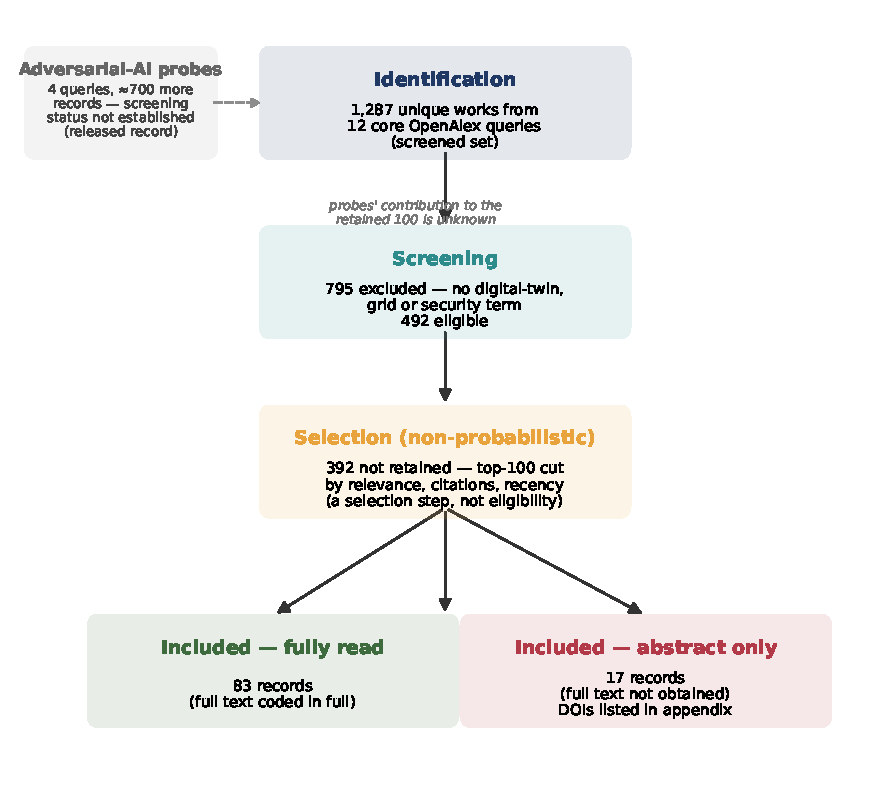
\includegraphics[width=0.86\textwidth]{fig1_prisma}
\caption{PRISMA-style flow. Eighty-three records are coded at full text and 17 at abstract
level only, because their full text was not obtained.}
\label{fig:prisma}
\end{figure*}

\subsection{Extraction}

We extracted 46 fields per record. Extraction was computer-assisted but human-coded: a script
surfaced keyword hits and context snippets for each field, and every code was assigned by a
human reading those snippets in context. Keyword snippets were scored against the full text and
the surrounding paragraph, not the excerpt alone; reference lists and author biographies were
stripped before scanning, so absence claims rest on the surviving body text. The extraction is
reproducible from the coded excerpts and DOIs, which are released.

Of the 100 records, 83 were available in full text and coded in full; 17 were available only as
abstracts and were coded at abstract level only. All abstract-only fields that require full text are treated as
missing, not as zero, throughout. The 17\% unobtainability rate is
reported as a reproducibility finding in Section~\ref{sec:validity}. Where the results
sections cite a corpus record (e.g.\ \cite{ref59}), the bracketed number resolves to that
record's own bibliographic entry; corpus record IDs used in tables are record numbers in the
released extraction matrix.

\subsection{Codebook}

The codebook defines each field and its controlled vocabulary, and was revised five times during
extraction. The revisions are logged in the repository and are load-bearing:

\begin{itemize}
  \item \textbf{R2} distinguishes a review from an enabling paper, and classifies
  attack-generating work as \emph{bridge}.
  \item \textbf{R3} requires a named interface or protocol before \texttt{attack\_surface\_named}
  may be coded \emph{yes}; passing mentions do not qualify.
  \item \textbf{R4} prevents passing mentions from triggering the \emph{multi} lifecycle value.
  \item \textbf{R5} contracts \texttt{ml\_family} to a controlled vocabulary.
  \item \textbf{R6} fixes evaluation-method precedence (\textit{hardware-in-the-loop} $>$
  testbed $>$ simulation) and maps surveys to \emph{concept} maturity.
\end{itemize}

All five revisions were applied retrospectively to all 100 records, not only to records
coded after each revision.

The \texttt{twin\_role} field requires positive evidence. \emph{both} needs explicit coverage of
the defensive and attack-target roles \emph{and} of the tension between them; \emph{target}
requires that the twin be the adversary's objective rather than an asset to be protected.
\emph{both} $= 0$ is therefore definitional: a paper cannot score \emph{both} without stating
the tension. Candidates such as \cite{ref84}, ``Enhancing the cybersecurity of battery digital
twins,'' were read as \emph{tool} because the twin remains an asset under protection.

\subsection{Scoring of AI-threat engagement}

Each AI-enabled threat field was coded on a 0--2 ordinal scale: 0 = not addressed; 1 =
mentioned, listed, or peripheral (fewer than two sentences or no failure-mode detail);
2 = substantive (a threat model, mechanism, experiment, or mitigation specific to that
vector, or a section dedicated to it). The threshold was applied to the full text rather than
the abstract. \texttt{ai\_threat\_overall} is 1 if any vector is 1 or 2, and 2 if any vector
is 2. Both coders coded the scale independently; per-vector agreement is reported in
Section~\ref{sec:agreement}.

\subsection{Reliability}\label{sec:reliability}

A second coder independently coded a 20\% random sample (20 studies) blind to coder 1's values
and to the screening label. Agreement is reported field by field in Section~\ref{sec:agreement}.
We use Cohen's $\kappa$ where it is defined and percentage agreement where a field is
near-constant and $\kappa$ is undefined. With $n = 20$, the large-sample standard error of
$\kappa$ is of the order of 0.2--0.3 even for the better fields; cells in Table~\ref{tab:reliability}
are point estimates, and a stable ranking of field difficulty is not achievable from this sample.

\subsection{Adjudication}

All field-level disagreements were adjudicated against the codebook and the underlying evidence.
The rules, stated here rather than buried, are: adopt the value the codebook and evidence
dictate; where both coders' values are defensible, coder 1's prevails; where neither fits, the
codebook rule decides. Adjudication changed 20 net cells, none of them a headline field
(Section~\ref{sec:agreement}). Because coder-1 precedence is a real limitation of the agreement
analysis, we report the raw agreement before adjudication alongside the adjudicated result.

\subsection{False-negative audit}

Because the headline is an absence---of attack-side engagement---we audited it. We ran a strict
AI-threat lexicon over the 48 records coded as \emph{not engaging} any AI threat and a broader
eleven-family net. The audit is reported in Section~\ref{sec:audit}; it bounds the false-negative
channel without eliminating it, and we say so.

\subsection{Verification and reproducibility}

Every DOI was verified against an authoritative registry: 96 of 97 resolved with a
title match (95 exact, one near), one DOI is not registered, and three corpus records carry no
DOI. Corpus metadata was cross-checked against Crossref, and 18 of 54 venue labels disagreed,
which we resolved in favour of the registry. All extraction data, the codebook, the coding
sheets, the reliability script, and the figure script are released as a reproducibility package.

\section{Results}\label{sec:results}

\subsection{Which denominator supports which claim}
Table~\ref{tab:denom} summarises the denominators behind the headline figures.
\begin{table}[t]
\centering
\caption{Denominators used in this review. The retained corpus, full-text and
abstract-only rows are corpus subsets; the remaining rows are subsets of the 83
full-text records.}
\label{tab:denom}
\small
\begin{tabular}{@{}lr@{}}
\toprule
Subset & $n$ \\
\midrule
Retained corpus & 100 \\
Full-text records & 83 \\
Abstract-only records & 17 \\
ML-used studies (full text) & 70 \\
Non-review studies (full text) & 49 \\
Journal articles (full text) & 62 \\
\bottomrule
\end{tabular}
\end{table}

The 62 journal articles are the full-text journal articles: 67 corpus journal articles
minus the five available only as abstracts.

\subsection{Corpus profile (RQ1, descriptive)}

The corpus is 100 studies: 67 journal articles, 17 conference papers, 5 theses, 4 preprints, 4
reports, and 3 book chapters. Publication is recent and accelerating: 1 study from 2020, 5 from
2021, 2 from 2022, 8 from 2023, 8 from 2024, 31 from 2025, and 45 from 2026; 76\% of the corpus
appeared in 2025 or 2026 (Figure~\ref{fig:yearvenue}a). The leading publishers are MDPI (17),
Elsevier (12) and IEEE (8); 42 records carry no publisher label in the source metadata.
Table~\ref{tab:profile} gives the profile.

\begin{figure*}[t]
\centering
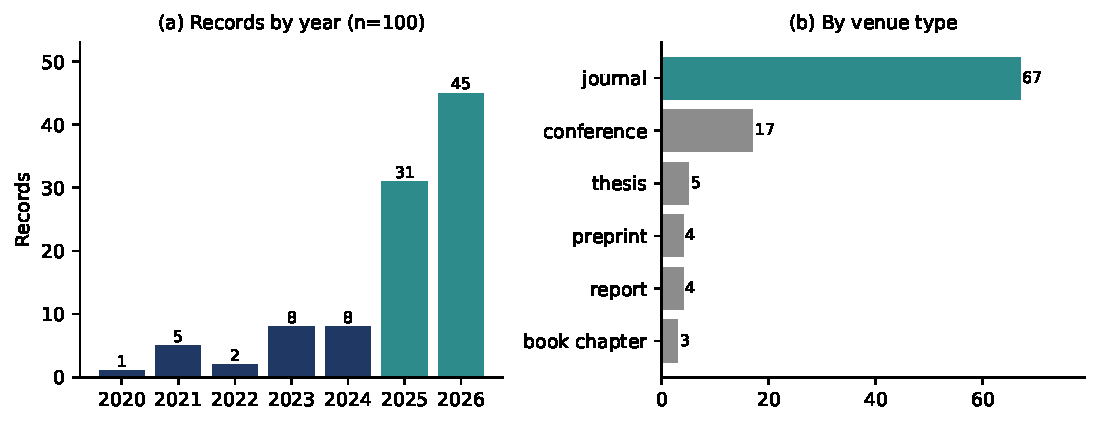
\includegraphics[width=0.92\textwidth]{fig2_year_venue}
\caption{Corpus profile. (a) Records by year. The 2025--2026 concentration reflects selection as much as
literature growth, since the top-100 cut favours recency among tied relevance scores.
(b) Records by venue type.}
\label{fig:yearvenue}
\end{figure*}

\begin{table}[t]
\centering
\caption{Corpus profile ($n=100$; full text $=83$, abstract-only $=17$).}
\label{tab:profile}
\small
\begin{tabular}{@{}lr@{}}
\toprule
Characteristic & Records \\
\midrule
Journal article & 67 \\
Conference paper & 17 \\
Thesis & 5 \\
Preprint & 4 \\
Report & 4 \\
Book chapter & 3 \\
\midrule
2026 & 45 \\
2025 & 31 \\
2024 & 8 \\
2023 & 8 \\
2022 & 2 \\
2021 & 5 \\
2020 & 1 \\
\midrule
Stance: defensive & 42 \\
Stance: review & 36 \\
Stance: bridge & 10 \\
Stance: enabling & 10 \\
Stance: adversarial & 2 \\
\bottomrule
\end{tabular}
\end{table}

\subsection{How the twin is positioned (RQ1)}

Across all 100 records, the adjudicated stance distribution is defensive 42, review 36, bridge
10, enabling 10, adversarial 2; security is the primary subject in 83 of 100
(Figure~\ref{fig:stance}a). The distribution differs from the screening seed---which had
adversarial 11, review 23---confirming that keyword-level stance labelling is unreliable and that
reading is necessary (Figure~\ref{fig:stance}b).

The sharper result is \texttt{twin\_role}, coded on the 83 full-text records: the twin is treated
as \emph{tool} in 75, as an attack \emph{target} in exactly 1 (Wilson 95\% interval 0--7\%), as \emph{both} in 0,
and is \emph{unclear} in 7. No paper in the corpus articulates the dual role that Habeeb et al.\
name \cite{habeeb2026}, and only one \cite{ref59} treats the twin as something to be attacked.
This is the first half of the asymmetry.

\begin{figure*}[t]
\centering
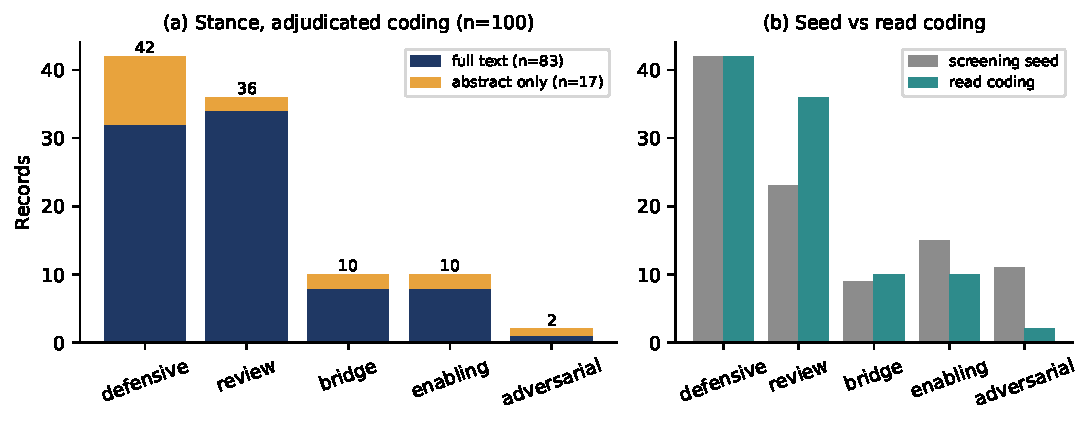
\includegraphics[width=0.92\textwidth]{fig3_stance}
\caption{Stance. (a) Adjudicated coding across all 100 records, split by whether full text was
coded. (b) Screening seed versus read coding: the shift from \emph{adversarial} to
\emph{review}/\emph{defensive} shows the seed over-called an adversarial stance on keyword
evidence.}
\label{fig:stance}
\end{figure*}

\subsection{Threat vocabulary and lifecycle concentration (RQ2)}

\label{sec:threats}
\label{sec:lifecycle}
Table~\ref{tab:threats} reports the closed threat vocabulary. Denial of service (49), false data
injection (46) and malware (34) lead; the AI-relevant terms that the corpus does contain---
poisoning (22), evasion (11)---are present but well behind the classical attacks. A mean of 3.77
distinct threats is named per full-text study (median 3, max 11), and 10 of 83 studies name no
threat at all, which is itself notable in a security review.

\begin{table}[t]
\centering
\caption{Threat vocabulary (full text, $n=83$). Terms are non-exclusive.}
\label{tab:threats}
\small
\begin{tabular}{@{}lr@{}}
\toprule
Threat & Records \\
\midrule
Denial of service (\texttt{dos}) & 49 \\
False data injection (\texttt{fdi}) & 46 \\
Malware (\texttt{malware}) & 34 \\
Man-in-the-middle (\texttt{mitm}) & 26 \\
Replay (\texttt{replay}) & 23 \\
False command injection (\texttt{false\_command}) & 22 \\
Data/model poisoning (\texttt{poisoning}) & 22 \\
Physical attack (\texttt{physical}) & 21 \\
Insider (\texttt{insider}) & 20 \\
Supply chain (\texttt{supply\_chain}) & 19 \\
Model evasion (\texttt{evasion}) & 11 \\
Reverse pathway (\texttt{reverse\_pathway}) & 10 \\
Other & 8 \\
Hardware & 1 \\
Prompt-level & 1 \\
\midrule
No threat named at all & 10 \\
Mean distinct threats per study & 3.77 \\
\bottomrule
\end{tabular}
\end{table}

Threat coverage is concentrated almost entirely at the operation phase.
Figure~\ref{fig:threatlife} crosses the threat vocabulary with \texttt{lifecycle\_stage}. The
design and commissioning columns are effectively empty---one design-phase study \cite{ref97} and
none at commissioning---while the operation column is dense. Across the corpus, lifecycle is
operation in 66 of 83 studies (79.5\%, Wilson 95\% interval 70--87\%), \emph{multi} in 12, unclear in 4, design in 1, and
commissioning in 0, as coded. Read as single labels, security work concentrates where the twin runs at deployment, not where it is built.

\begin{figure*}[t]
\centering
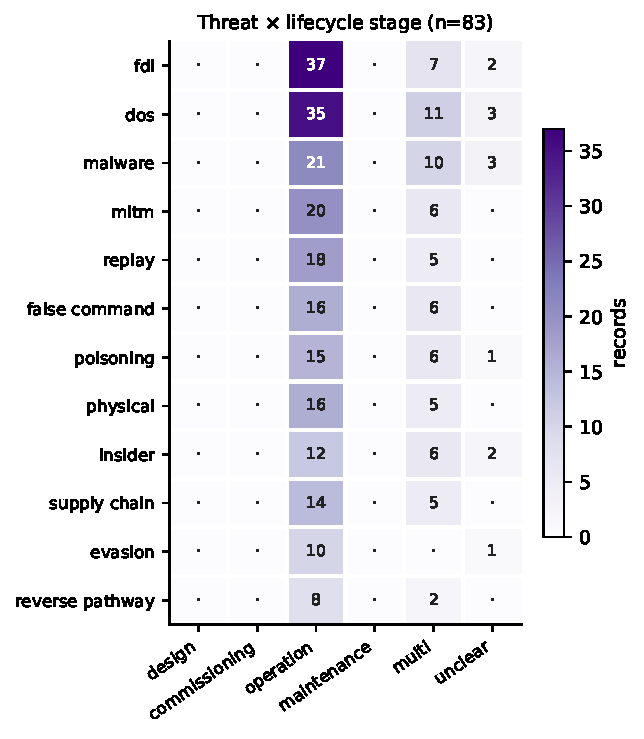
\includegraphics[width=0.6\textwidth]{fig4_threat_lifecycle}
\caption{Threat $\times$ lifecycle-stage coverage (full text, $n=83$). Empty cells in the design and
commissioning columns are a coding outcome, not a census of practice; the field's agreement is
$\kappa = 0.32$.}
\label{fig:threatlife}
\end{figure*}

Threat models are also thin. An explicit, stated threat model appears in 19 of 83 studies
(Wilson 95\% interval 15--33\%), and an adaptive adversary is modelled in 10 (7--21\%)---so the
corpus mostly names threats without committing to
an attacker model, which is precisely the weakness that makes attack-side claims hard to test.

\subsection{Engagement with AI-enabled threats (RQ3)}

\label{sec:ai-threats}
Note on terminology: the threat-vocabulary count (\texttt{poisoning}) and the AI-threat field
(\texttt{ai\_poisoning}) track different constructs; \texttt{poisoning} (22 records) records
any discussion of poisoning as a grid attack, while \texttt{ai\_poisoning} (19) records engagement
with AI-specific poisoning attacks.
This is the headline. Across the 83 full-text records, 35 (42.2\%, Wilson interval 32--53\%)
engage at least one AI-enabled threat at any level, 11 (13.3\%, 8--22\%) engage one
substantively, and 48 (57.8\%, 47--68\%) do not engage at all (Figure~\ref{fig:aithreats}). Restricting to the 49 non-review studies changes the counts but not the reading (20 of 49 engage
any, 6 of 49 substantively), so the asymmetry is not an artefact of review authorship.
Per vector, at any/substantive level: adversarial machine learning 24/8, data or model
poisoning 19/7, evasion 9/1, LLM-specific 4/2, and agentic attack automation 2/1. All 35 engaged studies are among the 70 that use machine learning defensively, so the
non-engagement is 35 of 70 (50\%) rather than a zero/one split. The asymmetry is real, but
it is an asymmetry of emphasis rather than absence.

\begin{figure*}[t]
\centering
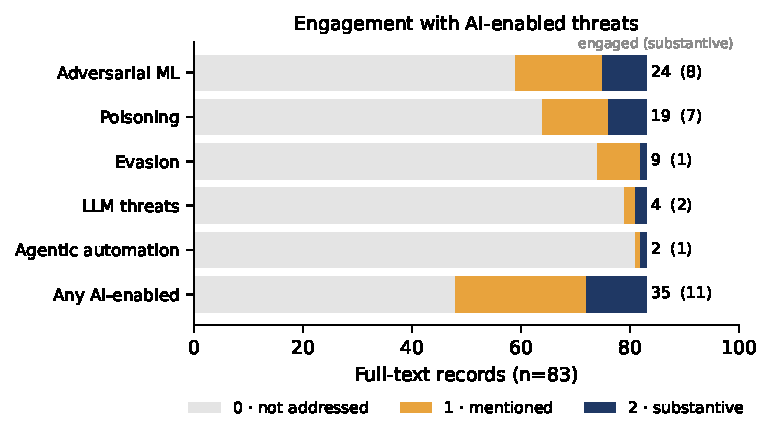
\includegraphics[width=0.82\textwidth]{fig5_ai_threats}
\caption{Engagement with AI-enabled threats (full text, $n=83$). Scale: 0 not addressed,
1 mentioned or peripheral, 2 substantive. The bar labels give engaged (substantive) counts.}
\label{fig:aithreats}
\end{figure*}

Two patterns sharpen the result. First, engagement is shallow: mentioned (score 1) is more
common than substantive (score 2) for every engaged vector except LLM threats (2 mentioned,
2 substantive, a tie on a base of 4) and agentic threats (1 mentioned, 1 substantive, a tie
on a base of 2). Second, the two deepest engagements are reviews \cite{ref16,ref50}; on the review authorship question
the substantive set has 5 reviews (45\%) against 34 (41\%) in the full-text base, i.e. no over-
representation; both counts are small and the difference is not statistically significant
(Fisher exact test, $p = 1.0$).

How much title-and-abstract screening loses on this question cannot be quantified from the
released record: an earlier abstract-level reading of a supplementary probe pool is not part
of the released corpus, and its denominator is therefore undefined here. What can be said is
directional. Engagement codes are assigned on full-text evidence, and records available only
as abstracts could not be scored at all, so abstract-only screening of this literature should
be expected to under-count AI-threat engagement relative to full-text coding.

Table~\ref{tab:substantive} lists the eleven substantive studies. Nine are journal articles (all 2025--26), one is a thesis \cite{ref74} and one a preprint
\cite{ref94} (2022); five carry the
\emph{review} stance and three the \emph{bridge} stance, so 8 of 11 are review-or-bridge work.
All eleven use ML predominantly for detection. No study's primary contribution is an
AI-enabled attack on a grid digital twin; the deepest engagements are themselves reviews
\cite{ref16,ref50}.

Read qualitatively, the eleven cluster into four patterns. (1) Generative and adversarial modelling as
attack generation: the twin is used to synthesise adversarially consistent attacks and GAN-based
evasion by the authors themselves \cite{ref16,ref24,ref49,ref50,ref57,ref94}. (2) Learned intrusion
detectors stressed under distribution shift: data poisoning \cite{ref17,ref74,ref94}, FGSM/JSMA
perturbations \cite{ref50}, and GAN-driven evasion \cite{ref49,ref94}. (3) LLM threats treated
as architecture-level hazards---hallucination, prompt injection, biased recommendations---in the
review literature \cite{ref16,ref24,ref50}. (4) Agentic automation represented only once, in
\cite{ref50}; no study constructs an adversarial RL or agentic pipeline. ``Substantive engage-
ment'' therefore currently means backgrounding a threat while retaining a defensive detector.

\begin{table*}[t]
\centering
\caption{The eleven studies engaging an AI-enabled threat substantively (score 2). IDs are corpus record numbers, not references. Vectors are non-exclusive. Qualitative pattern markers are in the prose above.}
\label{tab:substantive}
\small
\begin{tabular}{@{}rllll@{}}
\toprule
ID & Venue (type) & Year & Stance & AI-threat vectors \\
\midrule
16 & Energies (journal)                           & 2026 & review    & adv.\ ML, poisoning, LLM \\
17 & Sustain.\ Energy Technol.\ Assess.\ (journal) & 2026 & defensive & poisoning \\
22 & Informatics and Automation (journal)         & 2026 & bridge    & adv.\ ML \\
24 & Electronics (journal)                        & 2026 & review    & adv.\ ML, poisoning \\
49 & Sensors (journal)                            & 2025 & bridge    & adv.\ ML \\
50 & Energy Convers.\ Manag.\ X (journal)            & 2025 & review    & all five vectors \\
54 & Energies (journal)                           & 2025 & defensive & adv.\ ML \\
57 & Energies (journal)                           & 2025 & review    & poisoning \\
69 & Int.\ Res.\ J.\ Modernization (journal)      & 2025 & bridge    & adv.\ ML \\
74 & Deep Blue, Univ.\ Michigan (thesis)          & 2025 & defensive & poisoning \\
94 & arXiv (preprint)                             & 2022 & review    & adv.\ ML, poisoning \\
\bottomrule
\end{tabular}
\end{table*}

\subsection{Evidence quality (RQ4)}

Machine learning is used in 70 of 83 full-text studies; its dominant role is detection (55),
followed by forecasting (12), none (13), and control (3). Evaluation method splits as
simulation 33, qualitative 28, testbed 10, conceptual 5, mixed 5, and hardware-in-the-loop 2
(\cite{ref55,ref62} after adjudication). Maturity is prototype in 46, concept in 34, and
validated in only 3. Baselines are reported in 41 of 83 studies and quantitative metrics in 43,
while limitations are stated in 67. Code is released in 3 of 83 studies and data in 16. The
evidence base is, in short, prototyping-heavy and release-light. A venue-quality sensitivity
(restricting to the 62 full-text journal articles) leaves the asymmetry intact (26/62 any; 9/62 substantive;
36/62 none; 58/62 tool; twin targeted by one), though it discards 21 of the 83 full-text
records.
Restricting the denominators to the 49 non-review studies leaves the engagement result similar
(20/49 any versus 35/83) but not the baseline result: baselines rise from 41/83 (49\%) to 37/49
(76\%), and metrics from 43/83 (52\%) to 40/49 (82\%). Code and data remain low in both cases.

Grid domains are dominated by studies that span multiple domains (\emph{multi}, 47). Where a
single domain is named: distribution 11, unclear 7, EV charging 6, microgrid 6, transmission 5,
and substation 1. Transmission---often assumed to be the security-critical domain---is
under-represented relative to distribution and EV charging.

\subsection{Reliability results}

\label{sec:agreement}
Table~\ref{tab:reliability} reports agreement on the 20\% sample. On \texttt{ai\_threat\_overall}, the 3x3 counts are (rows coder 1, columns coder 2):
0: 9, 1, 1; 1: 1, 3, 1; 2: 1, 2, 1. Collapsing to ``any engagement vs. none'': coder 1 has
9 of 20, coder 2 has 9 of 20, agreement 16/20 ($\kappa$ = 0.60). Collapsing to
``substantive vs. not'': agreement 15/20, but $\kappa = 0.14$, because only 1 of the 6 studies is labelled substantively by both coders (the single (2,2) cell).
Under an asymptotic interval on this n = 20 sample, the 95\% interval is [-0.52, 0.79] for the
substantive collapse and [0.24, 0.95] for the any-engagement collapse; the two are not comparably
reliable.
This paragraph is a post-hoc reading of the 3x3 once we saw it, and is flagged as such. The disagreement on ``any engagement'' is symmetric (2 each way), so there is
no evidence that 35/83 is an undercount; the headline supported by the data is the 35/83 any,
not the 11/83 substantive, which is fragile.\par\vspace{0.5em}

Fields with substantial
agreement include \texttt{baseline\_compared} ($\kappa = 0.90$), \texttt{twin\_role} (0.77),
\texttt{ai\_poisoning} (0.73), \texttt{threat\_model\_explicit} (0.69) and
\texttt{metrics\_reported} (0.68). Fields at moderate or fair agreement include the ones the
headline most needs: \texttt{ai\_threat\_overall} (0.41), \texttt{ai\_evasion} (0.39), and the
threat-vocabulary fields. \texttt{attack\_surface\_named} is the weakest (0.14). Where a field is
near-constant, $\kappa$ is undefined and we report percentage agreement instead:
\texttt{stance\_confidence}, \texttt{limitations\_stated}, \texttt{data\_available},
\texttt{ai\_llm}, \texttt{ai\_agentic} and \texttt{code\_available}.

We report these numbers because they bound the result. The headline's core count---whether a
study engages any AI-enabled threat---is coded at only moderate agreement (0.41), so the 35/83 figure
carries real uncertainty. Two things mitigate it: adjudication moved no headline field, and the
false-negative audit (Section~\ref{sec:audit}) finds the absence robust under two independent
lexicons. But the honest reading is that the asymmetry's \emph{direction} is well supported while
its \emph{exact magnitude} should be quoted with care, and we do.

A systematic style difference between coders emerged and is worth recording as a codebook
problem rather than a coder problem: coder~1 tends to assign the default category
(\emph{high}, \emph{yes}, \emph{operation}, \emph{single}) whereas coder~2 differentiates
(\emph{medium}, \emph{no}, \emph{multi}, \emph{unclear}) and names more attack surfaces. Where
this is a default-category artefact, it depresses $\kappa$ without indicating a substantive
disagreement.

\begin{table}[!htbp]
\centering
\caption{Inter-coder agreement on the 20\% blind sample ($n=20$). $\kappa$ is reported where
interpretable; $\dagger$ marks near-constant fields (modal category $\ge 90$\% in coder 1)
where $\kappa$ is not interpretable and percentage agreement is reported instead.}
\label{tab:reliability}
\small
\begin{tabular}{@{}lcc@{}}
\toprule
Field & \% agree & $\kappa$ / set metric \\
\midrule
\multicolumn{3}{@{}l}{\textit{Cohen's $\kappa$ interpretable}} \\
baseline\_compared & 95 & 0.90 \\
twin\_role & 95 & 0.77 \\
ai\_poisoning & 90 & 0.73 \\
threat\_model\_explicit & 90 & 0.69 \\
metrics\_reported & 85 & 0.68 \\
security\_primary & 85 & 0.58 \\
ml\_used & 85 & 0.57 \\
ml\_role & 70 & 0.55 \\
stance & 60 & 0.46 \\
dt\_type & 75 & 0.46 \\
grid\_domain & 65 & 0.44 \\
ai\_adv\_ml & 70 & 0.44 \\
maturity & 60 & 0.42 \\
\textbf{ai\_threat\_overall} & \textbf{65} & \textbf{0.41} \\
ai\_evasion & 75 & 0.39 \\
eval\_method & 50 & 0.37 \\
lifecycle\_stage & 65 & 0.32 \\
attack\_surface\_named & 60 & 0.14 \\
\midrule
\multicolumn{3}{@{}l}{\textit{Percentage agreement only ($\dagger$)}} \\
code\_available & 100 & $\dagger$ \\
ai\_agentic & 95 & $\dagger$ \\
ai\_llm & 90 & $\dagger$ \\
data\_available & 85 & $\dagger$ \\
stance\_confidence & 70 & $\dagger$ \\
limitations\_stated & 70 & $\dagger$ \\
\midrule
\multicolumn{3}{@{}l}{\textit{Multi-label fields (set metrics)}} \\
threat\_models\_named & 5 & Jaccard 0.43 \\
ml\_family & 20 & Jaccard 0.30 (0.42 norm.) \\
threat\_count & 10 & mean $|\Delta|$ 1.80 \\
\bottomrule
\end{tabular}
\end{table}

\subsection{False-negative audit}

\label{sec:audit}
The strict AI-threat lexicon flagged none of the 48 records coded as not engaging, which is
consistent with the coding. But the audit is not, on its own, confirmatory: as a positive control
the same lexicon recovers only 7 of 11 known-positive studies, because some positives use generic
vocabulary the lexicon lacks (e.g.\ \cite{ref17,ref22,ref57,ref69}). A pattern set cannot
recognise wording it was not written for.

We therefore also ran a broader eleven-family net. Of the 48 negatives, 38 fired on some family
and 23 fired on a strong family. Inspection shows all 23 to be either conventional cyberattacks
discussed without any AI component or known false positives. The instructive false positives
justify human coding over keyword coding: \texttt{GaN} (the semiconductor) matching ``GAN'' in
two records \cite{ref41,ref84}, the author surname ``Gan'' in another \cite{ref90},
Xenon-135 reactor physics matching ``poisoning'' \cite{ref34}, ARP poisoning \cite{ref68}, and
the SolarWinds incident discussed as a data-poisoning example \cite{ref64}. Two close calls were
examined and cleared: \cite{ref86} bypasses \emph{classical} state-estimation bad-data detection,
not an ML detector, and \cite{ref15} concerns a SCADA supervisor with AI detection stated only as
future work. No codes were changed. The audit bounds but does not eliminate the false-negative
channel, because no lexicon matches wording it does not contain.

\subsection{Adjudication outcome}

Adjudication resolved 149 field-level disagreements and changed 20 net cells from coder~1's
values: \texttt{ml\_family} (12), \texttt{threat\_models\_named} (2), \texttt{stance} (2),
\texttt{eval\_method} (2), \texttt{dt\_type} (1) and \texttt{grid\_domain} (1). Three substantive
corrections came out of it: two studies move to \emph{bridge} stance \cite{ref22,ref49}, and one
study is a substation-domain study \cite{ref62}, contrary to its initial coding. Two third-value
resolutions occurred, both \texttt{eval\_method} $=$ hardware-in-the-loop \cite{ref55,ref62}.
No headline field moved, which is the point: the central result is not an artefact of the
tie-break rule.

\section{Discussion}\label{sec:discussion}

\subsection{The asymmetry, quantified}

The corpus adopts AI defensively in 70 of 83 full-text studies and engages AI-enabled threats in
35, substantively in 11. That gap---between near-universal defensive use and minority attack-side
engagement---is the paper's central finding, and it is robust to adjudication and to the
false-negative audit in direction if not in exact size. The practical reading is that the field
has built a large defensive apparatus on models whose own failure modes it rarely studies.

\subsection{The twin as a target is thinly evidenced}

As it stands, only one of our 83 full-text studies treats the twin as the adversary's
objective \cite{ref59}, and it concerns vehicle twins rather than grids. Habeeb et al.\ name
the twin as an expanded attack surface \cite{habeeb2026}; we cannot speak to that broader
version with a coding rule defined as ``the adversary's objective,'' so the grid-side evidence
for attack-surface engagement is, on these definitions, all but absent.

\subsection{The lifecycle blind spot is the deeper problem}

The result with the longest reach in the data, if it holds, is the lifecycle concentration:
66 of 83 studies are coded at the operation phase, one at design, none at commissioning. Two
caveats apply. First, the field carries our lowest inter-coder agreement ($\kappa = 0.32$), and
coder 1, who was the sole coder for 80 of the 100 records, defaults to `operation'; the 12 studies coded `multi'
may contain design or commissioning activity that the single label suppresses. Second, the score
records the phase a study 
\emph{targets}, not the phases it necessarily 
\emph{touches}. Read conservatively, the finding is therefore that the literature is dominated
by studies of running twins, with almost no study that sets out to secure a twin before it is
built, not that no design-phase security work exists.

\subsection{Why reviews are where the threats are named}

The two deepest engagements are reviews \cite{ref16,ref50}; 5 of the 11 substantive 
studies (45\%) are reviews against 34 of 83 (41\%) in the full-text corpus, so review 
authorship is not over-represented (Fisher exact test, $p = 1.0$), but bridge studies are
more prevalent (3 of 11 against 8 of 83 full-text records, 2 more in the abstract-only set;
Fisher exact test, $p = 0.12$, not significant at this $n$).
The honest reading is that reviews have the length and the licence to survey AI threats, while
primary papers have neither. Document length is a clear confound and these numbers should not
be read as evidence that 'only reviewers care.'

\subsection{Positioning against the prior review}

Relative to Habeeb et al.\ \cite{habeeb2026}, our contribution is a grid-side probe of a
narrower instance of one of their axes, with a published corpus, a closed vocabulary, and
reported reliability; full scope alignment is in Section~\ref{sec:bridge}. Table
\ref{tab:bridge} shows that our independent vocabulary covers all five of their vectors, so the
comparison is not competing but additive. Two caveats are structural, not rhetorical. First,
their search string has no specific attack-side operator, so records enter only through
security terms; ours adds four
adversarial-AI probes and still finds shallow engagement, so the gap is not merely their
query's doing. Second, their corpus spans manufacturing, healthcare, water and smart city, where
the digital twin's role differs from the grid's bidirectional, safety-critical loop; grid
conclusions should not be generalised from it, nor it from us.

\subsection{Operational reading}

For operators, three interpretive notes follow (these are author readings, not coded evidence).
First, a twin whose learner is trained on the same telemetry it is meant to defend has no
independent ground truth and is a single point of failure that the corpus rarely names.
Second, runtime detection at the operation phase is necessary, but cannot cover design-stage
trust failures. Third, the near-total absence of released code and data means a twin
procurement decision cannot currently be informed by reproducible attack evidence.

\section{Research agenda}\label{sec:agenda}

We state five items. Each is tied to the gap that justifies it (from Section~\ref{sec:results})
and to the validation that would confirm it, so the agenda is testable rather than aspirational.
Table~\ref{tab:agenda} summarises.

\begin{description}
  \item[P1 --- Measure the twin as an attack target, not only as a defence.]
  Justified by \texttt{twin\_role} target $=1$; validated by a reproducible attack against a
  grid twin where the twin is the objective, with released code and a stated adaptive adversary.
  \item[P2 --- Move security to design and commissioning.]
  Justified by operation $=66$, design $=1$, commissioning $=0$; validated by twins whose trust
  boundaries, interface contracts and fail-safe behaviour are specified and tested before
  deployment.
  \item[P3 --- Adopt explicit adaptive threat models.]
  Justified by an explicit threat model in 19/83 and an adaptive adversary in 10/83; validated by
  studies that state the attacker's knowledge, capability and objective and test a reactive
  attacker.
  \item[P4 --- Defend the learned components, not just the plant.]
  Justified by detection-dominant ML use (55/83) against shallow poisoning and evasion
  engagement (22 and 11); validated by poisoning- and evasion-robust twins under distribution
  shift.
  \item[P5 --- Release code and data.]
  Justified by code in 3/83 (3/49 non-review) and data in 16/83; baseline disclosure alone is
  high among primary studies, but reproducibility remains impossible without code or data.
\end{description}

P5 must be stated carefully. We measure \emph{research attention}, not \emph{deployment security}.
A low attack-side count does not mean grids are undefended; it means the published research has
not modelled these attacks. We cannot estimate either the probability of an AI-enabled attack or
its expected impact from this corpus, and we do not.

\begin{table}[!htbp]
\centering
\caption{Research agenda: gap, direction, and the validation each item demands.}
\label{tab:agenda}
\small
\begin{tabular}{@{}p{0.6cm}p{3.4cm}p{4.4cm}p{5.2cm}@{}}
\toprule
\# & Gap (evidence) & Direction & Validation \\
\midrule
P1 & Twin as target: 1/83 & Treat the twin as the adversary's objective & Reproducible twin-directed attack with released code, adaptive adversary \\
P2 & Design 1/83, commissioning 0/83 & Secure design and commissioning phases & Trust boundaries and fail-safes specified and tested pre-deployment \\
P3 & Explicit threat model 19/83; adaptive 10/83 & State and test adaptive threat models & Attacker knowledge, capability, objective stated; reactive attacker tested \\
P4 & Poisoning 19, evasion 9 vs detection 55 & Defend learned components & Poisoning/evasion-robust twin under distribution shift \\
P5 & Code 3/83 (3/49 non-review), data 16/83 & Release artifacts & Third party reruns unaided \\
\bottomrule
\end{tabular}
\end{table}

\section{Threats to validity}\label{sec:validity}

\subsection{Construct validity}
``AI-enabled threat'' is a construct, and the false-negative audit shows a strict lexicon misses
some positives (7/11 recovery). We mitigated by human coding with context, by the broad
eleven-family net, and by the conservative \texttt{twin\_role} rule, but the construct remains
softer than the threat-vocabulary fields.

\subsection{Internal validity and screening}
Screening on title and abstract is imperfect, and for this corpus the loss is unquantified:
AI-threat engagement was scored on full text, the 17 abstract-only records could not be
scored on it at all, and the supplementary probe pool behind an earlier abstract-level reading
is not part of the released record, so no like-for-like comparison is offered. The direction
of the effect is clear---engagement signals frequently live in the body of a paper rather than
its abstract---so abstract-level screening of this literature should be read as a lower bound
on engagement.

\subsection{Reliability}
Agreement on headline fields is moderate, not strong (\texttt{ai\_threat\_overall} $\kappa = 0.41$;
\texttt{attack\_surface\_named} 0.14). Coder-1 precedence in adjudication is a real limitation
and is declared. The exact magnitude of the asymmetry should therefore be read with the
reliability table, not in isolation.

\subsection{External validity and coverage}
PRISMA compliance is partial: one database, no registered
protocol and five codebook revisions after the protocol was `fixed'---all of which limit how
strongly the review answers the protocol hypothesis. The search cutoff is stated in
Section~\ref{sec:method} (the corpus freeze date of 16 October 2026).\par\vspace{0.5em}
Seventeen of the 100 records were available only as abstracts, hence the corpus has a 17\%
non-full-text rate; those records are listed with DOIs so readers can check what is missing. One
corpus DOI does not resolve (record 18, which lies within the reliability sample) and three
records have no DOI; these are disclosed rather than dropped. Venue labels disagreed with
Crossref in 18 of 54 cases and were corrected in favour of the registry.

\subsection{Search bias}
The core grid-security vocabulary does not retrieve attack-side work; the four adversarial-AI
probes were added to widen the candidate pool (approximately 2,000 records), and the
released dataset does not carry per-record query provenance, so probe-only membership among
the retained 100 cannot be computed post hoc; this is a gap in
the record. Even with
them, engagement is shallow, so the asymmetry is not merely a retrieval artefact---but the corpus
should still be read as a bounded sample rather than a census. The recency component of the
ranking also means foundational attack-side work from 2020--2023 may be under-weighted.

\subsection{Researcher degrees of freedom}
Five codebook revisions during extraction are a real degree of freedom. They are logged, dated,
and applied consistently to all 100 records, and adjudication used the same rules; but a reader
who distrusts post-hoc refinement should weight the raw pre-adjudication codes, which are
released frozen alongside the adjudicated matrix.

\subsection{Quality appraisal, venue quality and scope}
At least one retained record \cite{ref18} carries anonymous authorship in a low-tier journal,
which is exactly why the venue sensitivity and DOI verification passes above were necessary.
The corpus contains 67 journal articles, 17 conference papers, 5 theses, 4 preprints, 4 
reports and 3 book chapters, drawn from venues of varying strictness (including IRJMETS and
GSC Online Press). No formal risk-of-bias or venue-quality appraisal was performed; all
prevalence figures are therefore reported over the full corpus, and Section~\ref{sec:results}
reports sensitivity subsets for non-review studies. Readers should weight venue quality into
any claim reproduced from this review. The claim in Section~1 is restricted to
the intersection of `digital twin' and `cybersecurity' in power grids; substantial 
adversarial-ML work on grid state estimation lies outside that intersection and is not covered
by the headline numbers.\par\vspace{1em}

\section{Conclusion}\label{sec:conclusion}

Grid digital-twin security has adopted AI as a defensive tool far faster than it has modelled
AI---or the twin itself---as an attack target. Across a screened corpus of 100 studies,
76\% published in 2025--26, AI is defensive in 70 of 83 full-text studies while 35 engage any AI-enabled threat and 11 engage
one substantively; the twin is an explicit attack
target in exactly one study under the strict codebook definition (a vehicle-twin review; the
count under a looser asset-under-protection definition is uncomputed). Coverage is dominated by the operation phase (66 of 83 coded as such, on a field with
$\kappa = 0.32$); at most, one study is coded at design and none at commissioning, and threat
models are thin (explicit in 19/83).
These directions are robust to adjudication and to a two-lexicon false-negative audit, though the
exact magnitudes are bounded by moderate coder agreement on the headline fields. The closest prior
review names the dual role; this review tests one of its axes at grid scale and finds it largely
empty. The five-item agenda that follows is deliberately testable: each item names the gap that
justifies it and the evidence that would close it.

\section*{Highlights}
\begin{itemize}
  \item 100-study review of digital twins for power-grid cybersecurity, 2020--2026.
  \item AI is defensive in 70/83; 35/83 engage an AI threat; 11/83 substantively (fragile).
  \item Only one study treats the twin itself as an attack target (strict definition).
  \item Coverage: 66/83 at operation, 1 at design, 0 at commissioning, as coded.
  \item Five-item agenda: each item names its gap and the evidence that would close it.
\end{itemize}

\section*{Declaration of competing interest}
The authors declare no competing interests.

\section*{Data availability}
All extraction data, the codebook, the coder sheets, the reliability script and the figure script
are available in the reproducibility package accompanying this review (repository link supplied
at submission).

\section*{CRediT authorship contribution statement}
\textbf{Author One:} conceptualisation, methodology, formal analysis, writing---original draft.
\textbf{Author Two:} validation, reliability coding, writing---review and editing.

\bibliographystyle{elsarticle-num}
\bibliography{included}

\end{document}
